\begin{figure}
\centering
    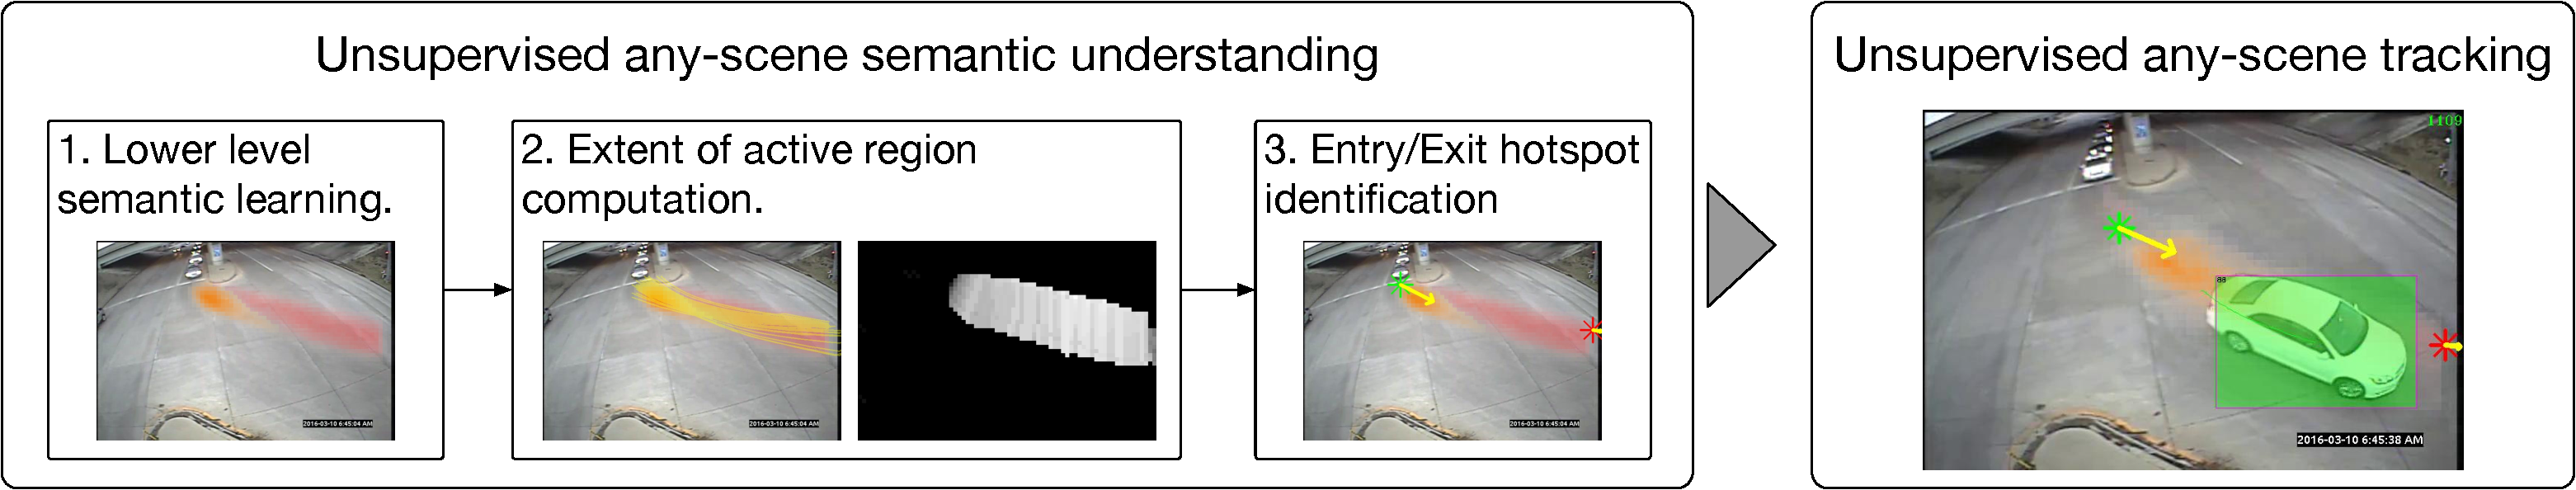
\includegraphics[width=\linewidth]{./img/scene_learning/workflow.pdf}
    \caption{System overview. The left corresponds to scene learning module: frequent motions are extracted in an unsupervised fashion, then the active regions where most objects move are learned on top of the motion result. Next, the entry/exit hotspot and their direction are extracted, describing how most objects enter and exit the scene. On the right, the semantic knowledge is applied to a tracker.}
    \label{fig:scene-workflow}
\end{figure}